\chapter{Results}
This section presents the results from the power consumption measurements. The results will be discussed and compared in terms of the different techniques used to make the game more power efficient.

The power consumption was examined with three different benchmarks. The first benchmark shows the power consumption without any sleep, and with the display refresh function set to refresh the entire display each time a change occurs. As seen from Figure \ref{fig:no_opt}, the average current consumption is 33mA.

\begin{figure}[h]
\centering
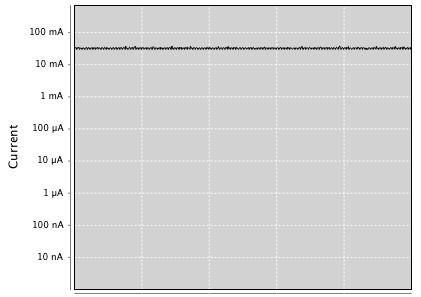
\includegraphics[width=0.5\textwidth]{images/welcome_no_opt.png}
\label{fig:no_opt}
\caption{Average current consumption of 33mA with game running with no optimizations.}
\end{figure}

The second benchmark shows the power consumption with sleep enabled in-between a display refresh. The display is still set to refresh the entire display when a change occurs. As seen from Figure \ref{fig:sleep}, the average current consumption is 30mA. This number underlines the cost of an entire display refresh.  

\begin{figure}[h]
\centering
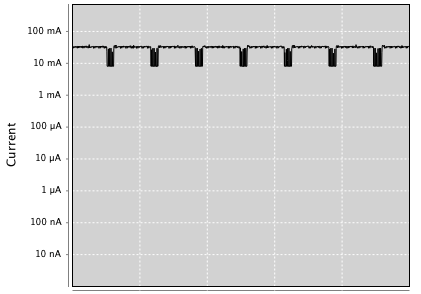
\includegraphics[width=0.5\textwidth]{images/welcome_sleep.png}
\label{fig:sleep}
\caption{Average current consumption of 30mA with game running with no optimizations but put to sleep for 50ms each iterations of main.}
\end{figure}

In the third and final benchmark shows the power consumption for our final implementation. Here, the application has been optimized to only refresh display sections that has movement. This makes the refresh procedure very fast, which in term enables us to hibernate the CPU for longer period of time. The results of this can clearly be seen from Figure \ref{fig:opt}, where the average current consumption is only at 12mA. 

\begin{figure}[h]
\centering
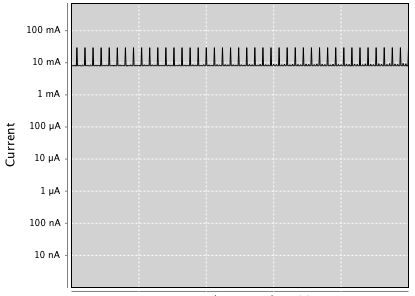
\includegraphics[width=0.5\textwidth]{images/welcome_opt.png}
\label{fig:opt}
\caption{Average current consumption of 12mA with game running with optimizations.}
\end{figure}

Pengutronix, the company responsible for porting uCLinux to the EFM32GG, claims that the distribution should be able to run as low 1.6mA in IDLE mode. Even with a lot of kernel configuration attempts, we were not able to achieve this number. 

\section{Kernel configurations}

Several kernel configuration was tested. Tickless kernel, opportunistic sleep and CPU power modes was enabled. However, none of the options gave any noticeable difference in the overall power consumption.  